\documentclass[12pt, a4paper, oneside]{book}
\usepackage[hidelinks]{hyperref}
\usepackage[english]{babel}
\usepackage{epsfig}
\usepackage{epstopdf}
\usepackage[chapter]{algorithm}
\usepackage{algorithmic}
\usepackage{listings}
\usepackage{amsmath}
\usepackage{dirtytalk}
\usepackage{amssymb}
\usepackage{graphicx}
\usepackage{multirow}
\usepackage{color}
\usepackage{url}
\usepackage[utf8]{inputenc}
\usepackage[T1]{fontenc}
\usepackage{setspace}
\usepackage{tabularx}
\usepackage{textcomp}
\usepackage{caption}
\usepackage{subfig}
\usepackage{natbib}
\usepackage{nopageno}


\setstretch{1.5}
%\renewcommand\baselinestretch{1.5} % riadkovanie jeden a pol

% pekne pokope definujeme potrebne udaje
\newcommand\mftitle{Algorithm development for the segmentation of astronomical images with unique features}
\newcommand\mfthesistype{Masters Thesis}
\newcommand\mfauthor{Bc. Viktor Nagy}
\newcommand\mfadvisor{prof. RNDr. Jiri Silha, PhD.}
\newcommand\mfplacedate{Bratislava, 2014}
\newcommand\mfuniversity{UNIVERZITA KOMENSKÉHO V BRATISLAVE}
\newcommand\mffaculty{FAKULTA MATEMATIKY, FYZIKY A INFORMATIKY}
\newcommand{\sub}[1]{$_{\text{#1}}$}
\newcommand{\reference}[1]{č.~\ref{#1}}
\newcommand{\imageHeight}{150px}

\ifx\pdfoutput\undefined\relax\else\pdfinfo{ /Title (mftitle) /Author (\mfauthor) /Creator (PDFLaTeX) } \fi

\begin{document}

\frontmatter

\thispagestyle{empty}

\noindent
\begin{minipage}{\textwidth}
\begin{center}
\textbf{\mfuniversity \\
\mffaculty}
\end{center}
\end{minipage}

\vfill
\begin{figure}[!hbt]
    \begin{center}
        
\includegraphics{images/logo_fmph}
        \label{img:logo}
    \end{center}
\end{figure}
\begin{center}
    \begin{minipage}{0.8\textwidth}
        \centerline{\textbf{\Large\MakeUppercase{Algorithm development for the segmentation}}}
        \centerline{\textbf{\Large\MakeUppercase{of astronomical images with unique features}}}
        \smallskip
        \centerline{\mfthesistype}
    \end{minipage}
\end{center}
\vfill
2014 \hfill
\mfauthor
\eject
% koniec obalu

\thispagestyle{empty}

\noindent
\begin{minipage}{\textwidth}
\begin{center}
\textbf{\mfuniversity \\
\mffaculty}
\end{center}
\end{minipage}

\vfill
\begin{figure}[!hbt]
\begin{center}

\includegraphics{images/logo_fmph_dark}
\label{img:logo_dark}
\end{center}
\end{figure}
\begin{center}
\begin{minipage}{0.8\textwidth}
        \centerline{\textbf{\Large\MakeUppercase{Algorithm development for the segmentation}}}
        \centerline{\textbf{\Large\MakeUppercase{of astronomical images with unique features}}}
\smallskip
\centerline{\mfthesistype}
\end{minipage}
\end{center}
\vfill
\begin{tabular}{l l}
%Registration number: & 40a99bd8-3cb6-4534-9330-c7fd9b5e5ca4 \\
Študijný program: & Aplikovaná informatika\\
Študijný odbor: & 2511 Aplikovaná informatika\\
Školiace pracovisko: & Katedra aplikovanej informatiky\\
Školiteľ: & \mfadvisor
\end{tabular}
\vfill
\noindent
\mfplacedate \hfill
\mfauthor
\eject
% koniec titulneho listu

%\thispagestyle{empty}
%\includegraphics[width=\textwidth]{images/zadanie}
%\vfill
%\eject
% koniec zadania



\begin{figure}[H]
\vspace*{-3.5cm}
\begin{center}
\makebox[\textwidth]{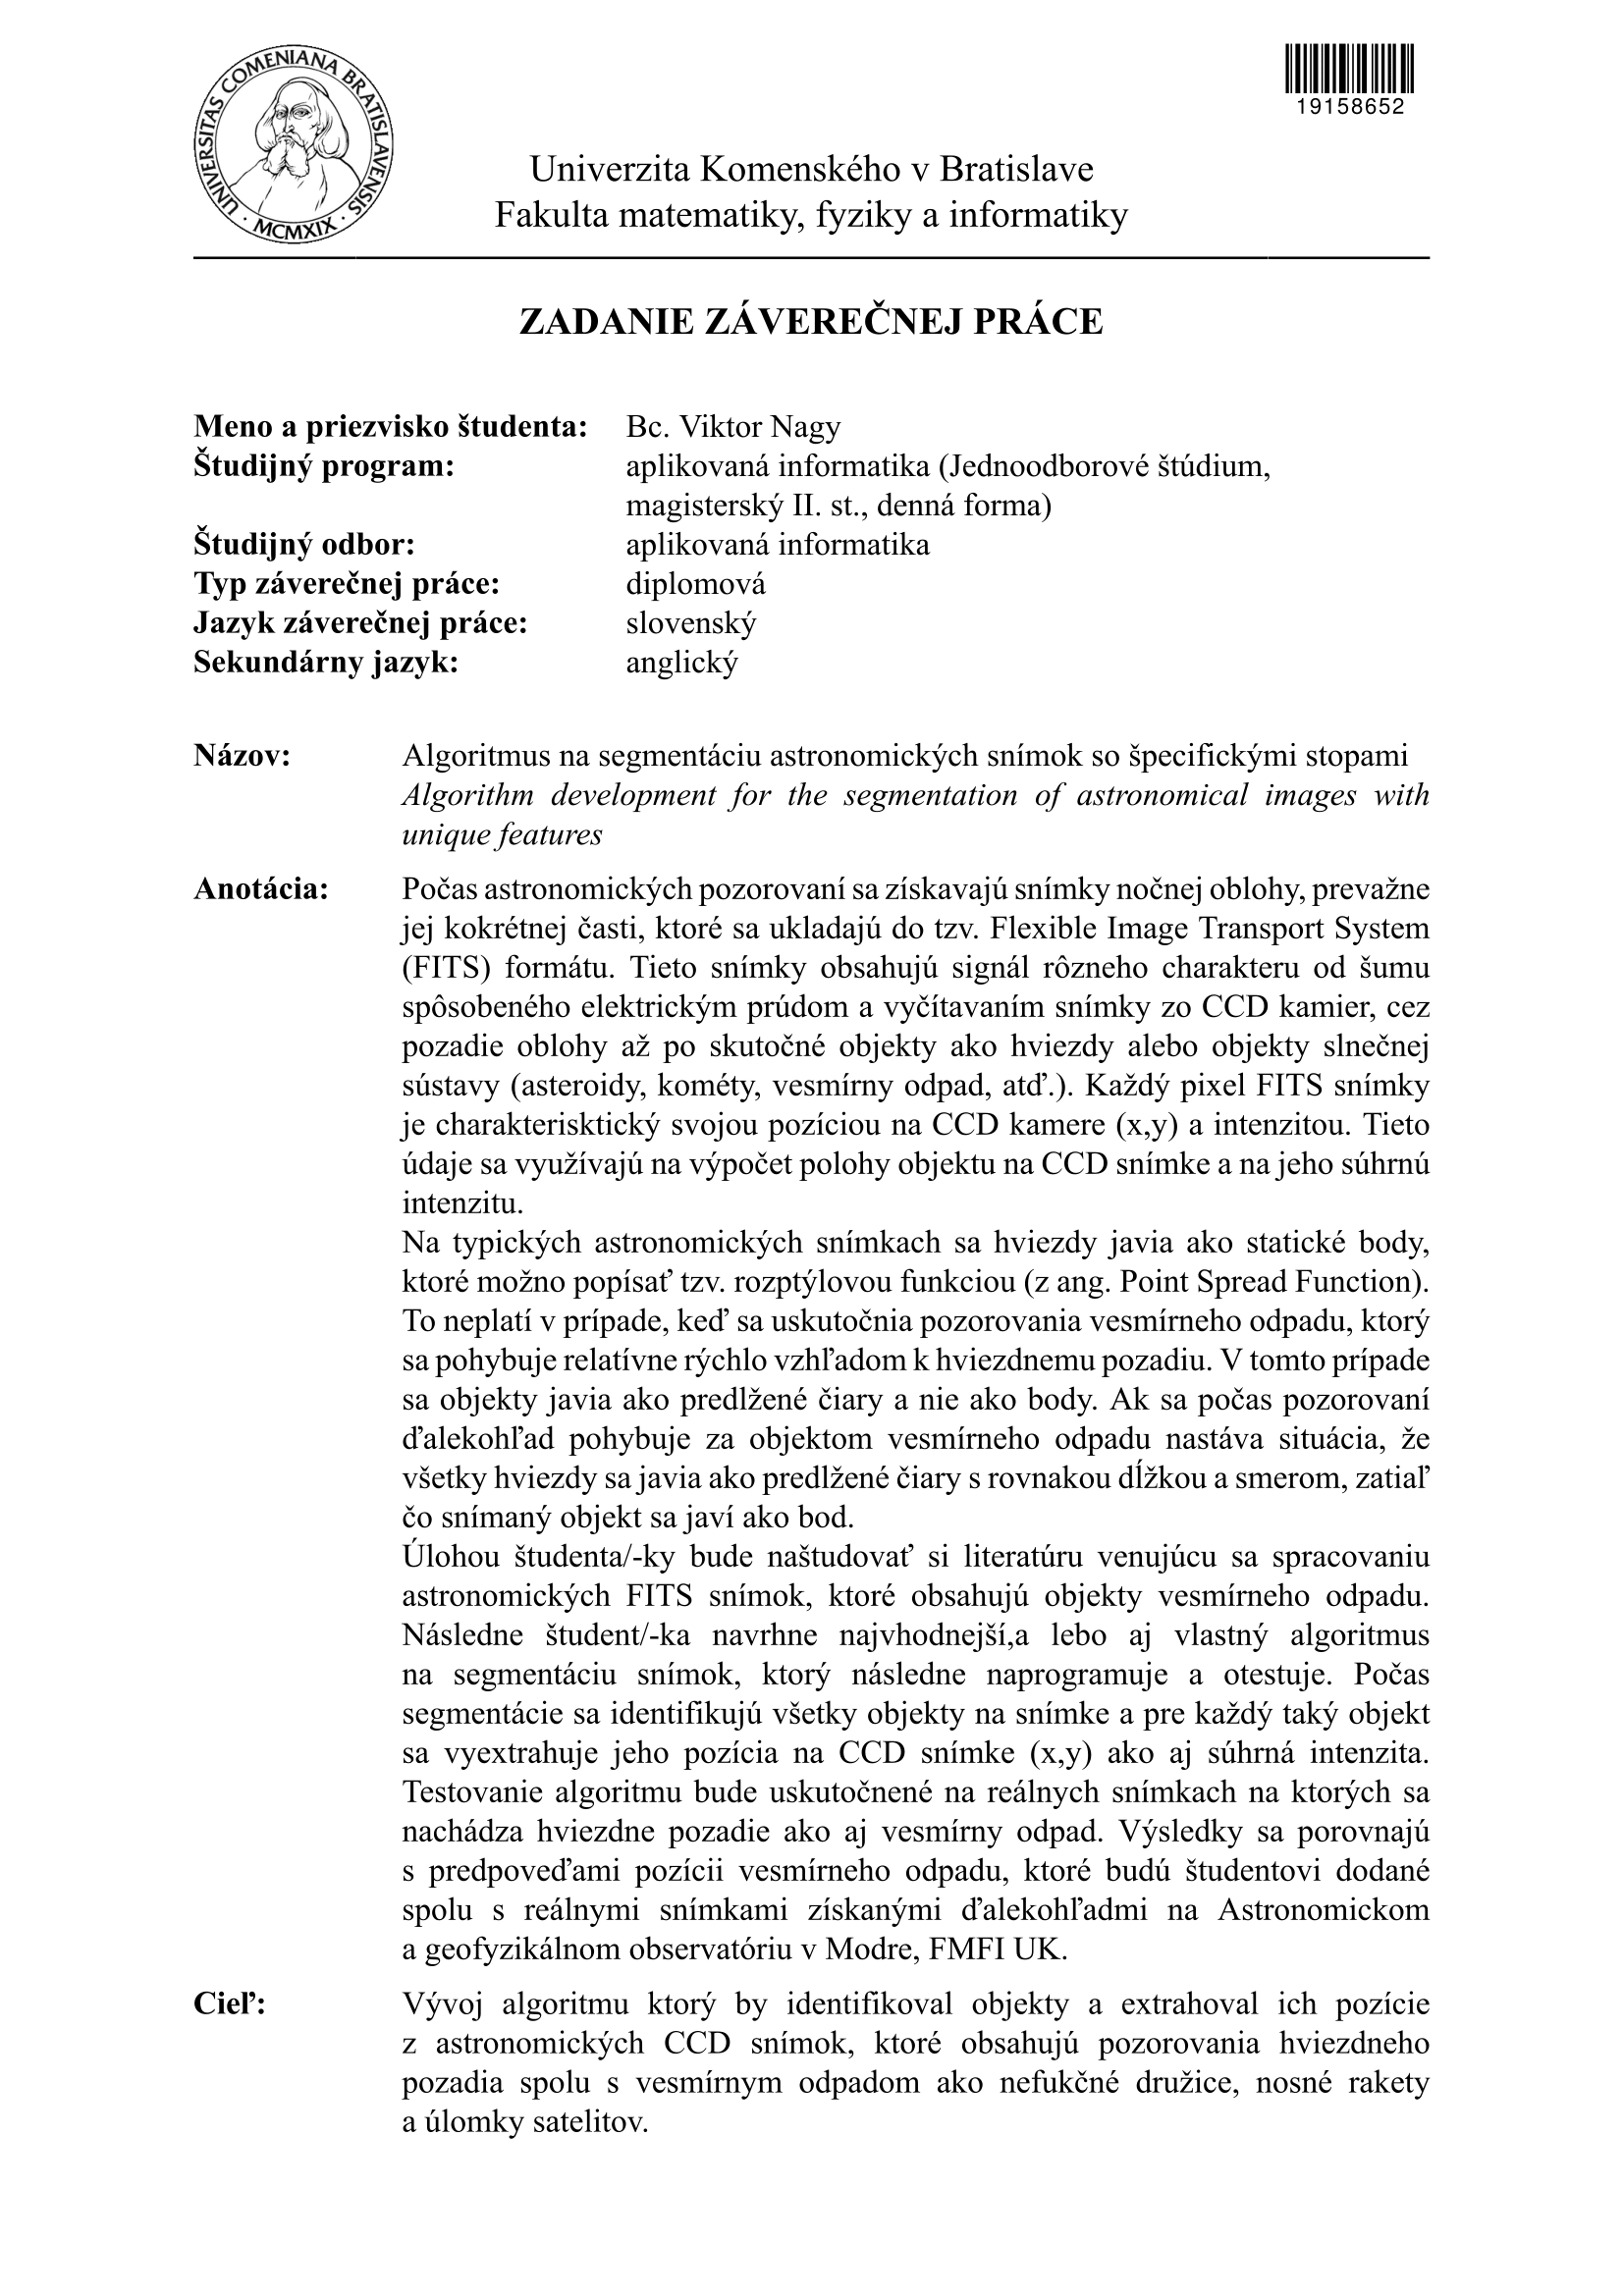
\includegraphics[width=\paperwidth]{zadanie1.png}}
\label{img:zadanie}
\end{center}
\end{figure}

\begin{figure}[H]
\begin{center}
\makebox[\textwidth]{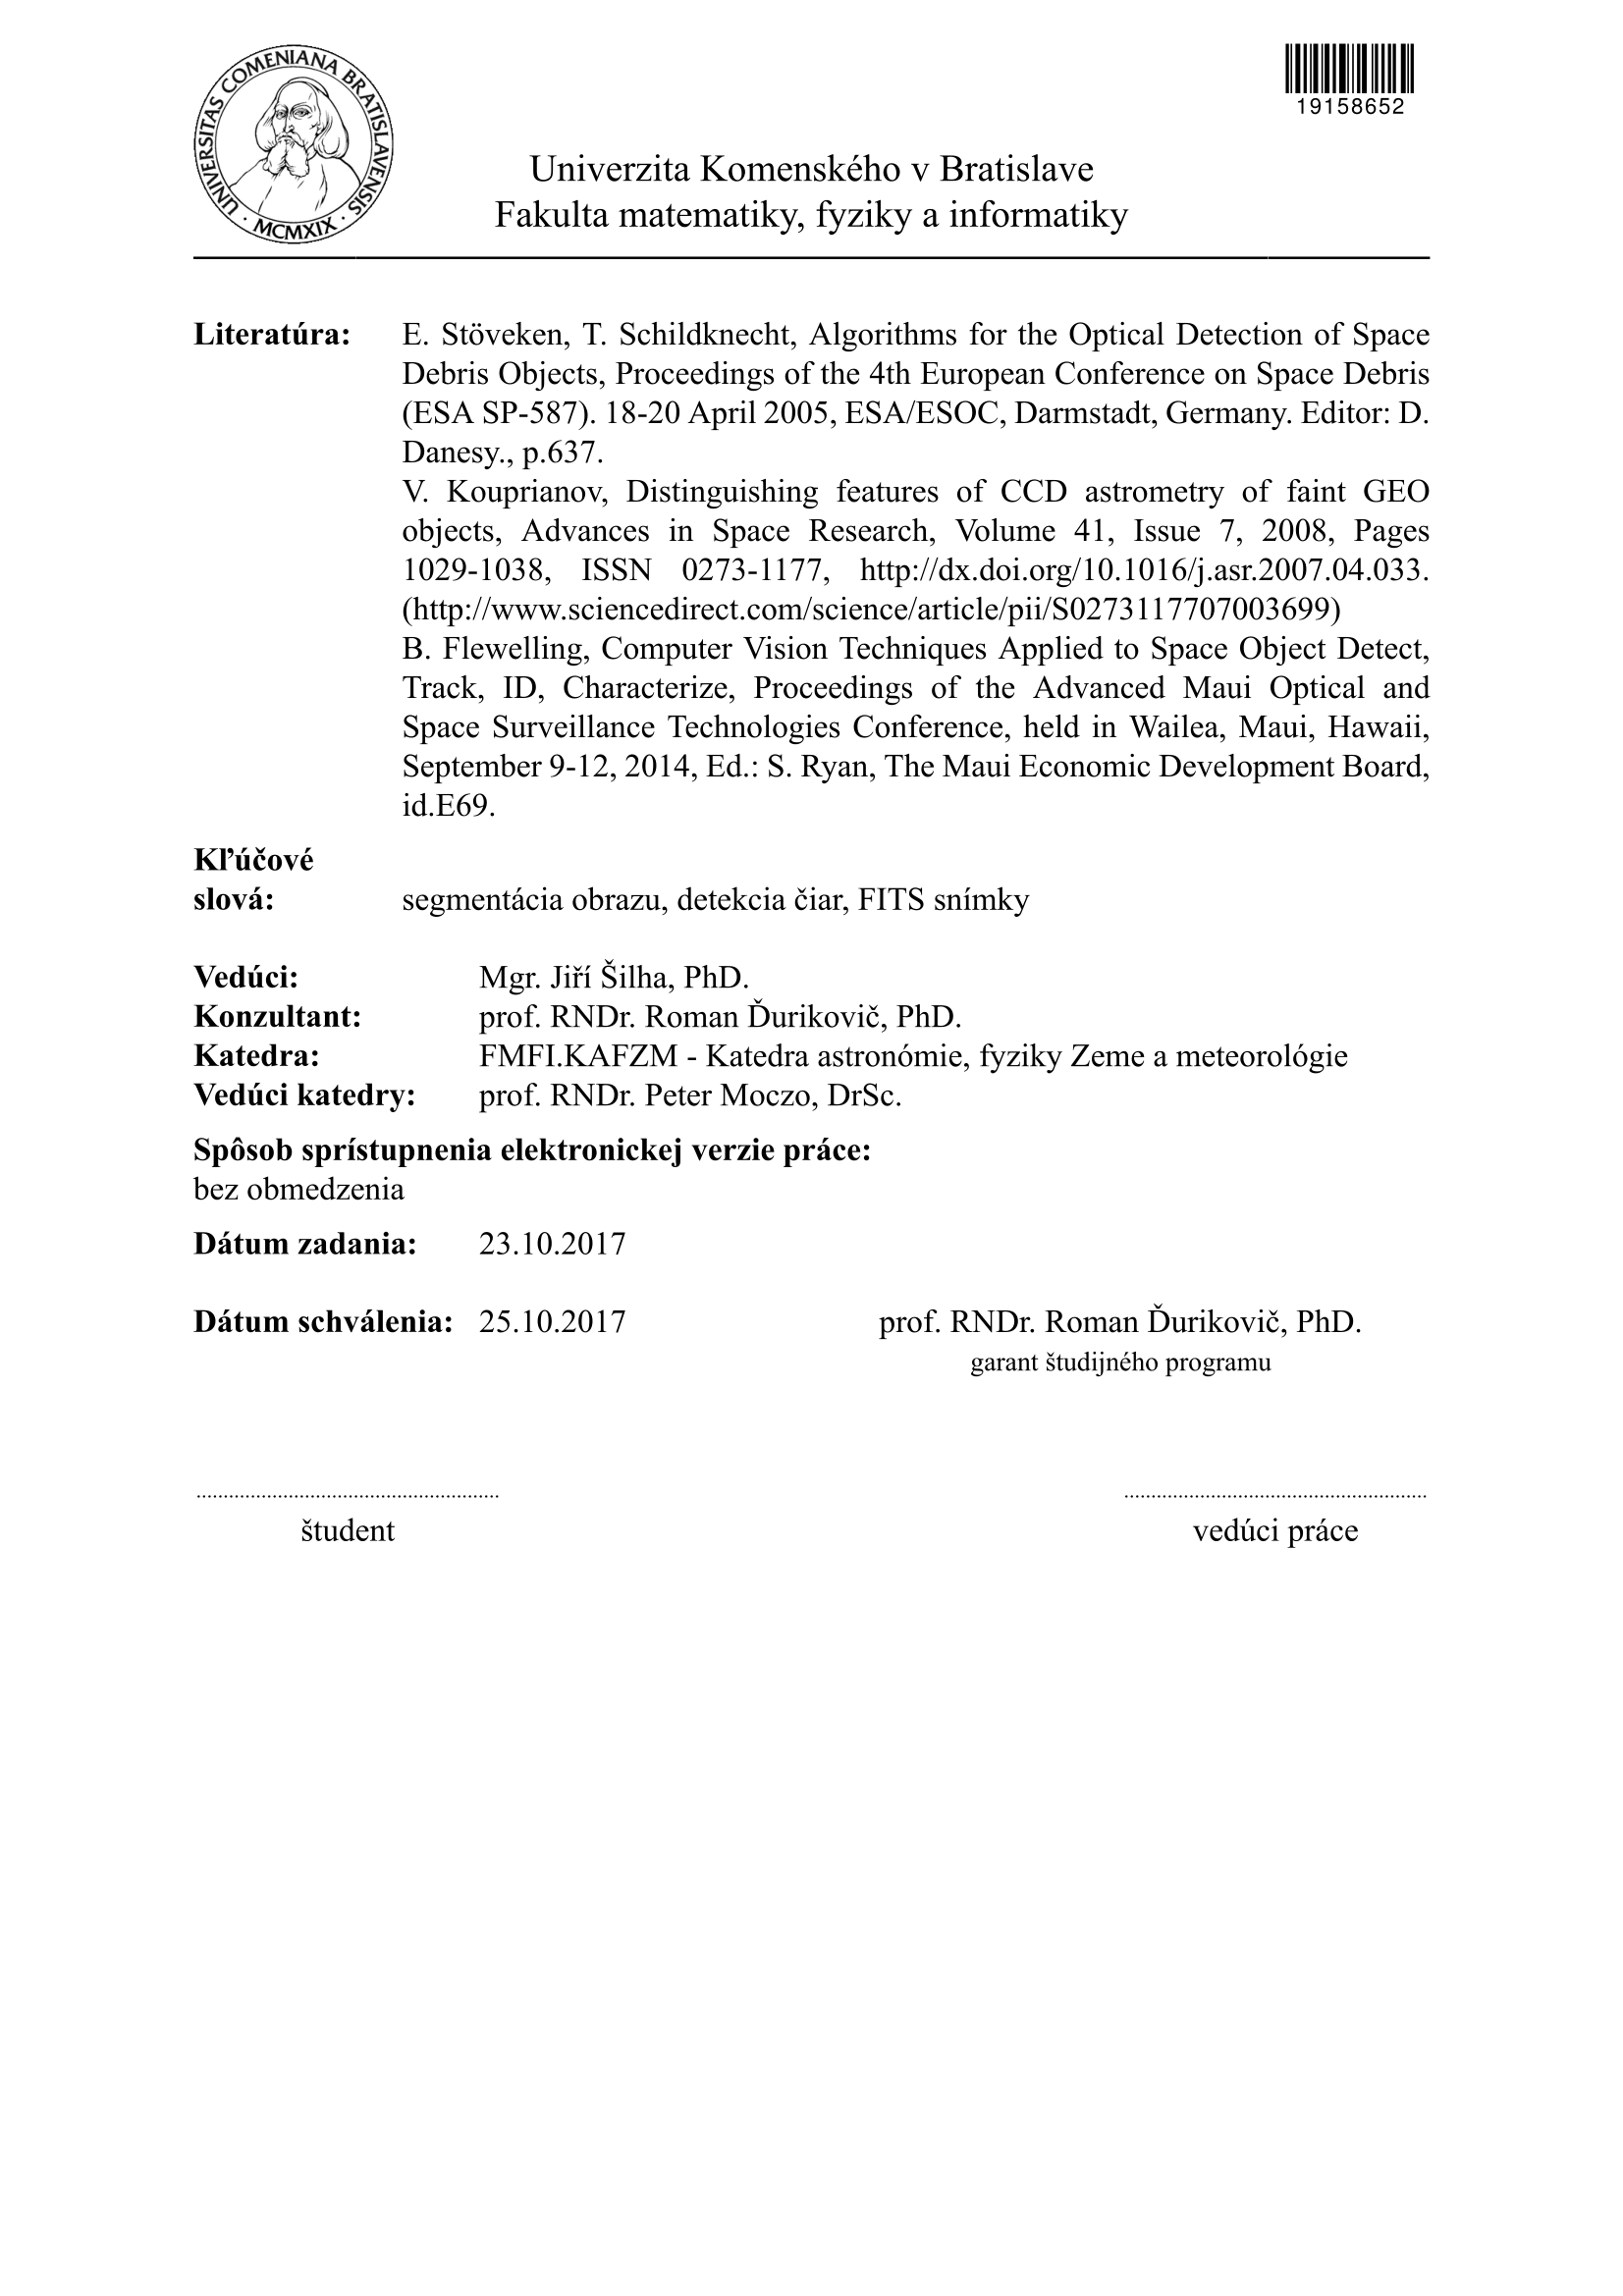
\includegraphics[width=\paperwidth]{zadanie2.png}}
\label{img:zadanie}
\end{center}
\end{figure}


\noindent
\begin{minipage}{0.25\textwidth}~\end{minipage}
\begin{minipage}{0.75\textwidth}
Čestne prehlasujem, že túto diplomovú prácu som vypracoval samostatne len s použitím uvedenej literatúry a za pomoci konzultácií u môjho školiteľa.
\newline \newline
\end{minipage}
\vfill
~ \hfill {\hbox to 6cm{\dotfill}} \\
\mfplacedate \hfill \mfauthor
\vfill\eject
% koniec prehlasenia

\chapter*{Poďakovanie}\label{chap:thank_you}
\vfill\eject
% koniec podakovania

\chapter*{Abstrakt}\label{chap:abstract_sk}
Počas astronomických pozorovaní sa získavajú snímky nočnej oblohy, prevažne jej kokrétnej časti, ktoré sa ukladajú do tzv. Flexible Image Transport System (FITS) formátu. Tieto snímky obsahujú signál rôzneho charakteru od šumu spôsobeného elektrickým prúdom a vyčítavaním snímky zo CCD kamier, cez pozadie oblohy až po skutočné objekty ako hviezdy alebo objekty slnečnej sústavy (asteroidy, kométy, vesmírny odpad, atď.). Každý pixel FITS snímky je charakterisktický svojou pozíciou na CCD kamere (x,y) a intenzitou. Tieto údaje sa využívajú na výpočet polohy objektu na CCD snímke a na jeho súhrnú intenzitu.
Na typických astronomických snímkach sa hviezdy javia ako statické body, ktoré možno popísať tzv. rozptýlovou funkciou (z ang. Point Spread Function). To neplatí v prípade, keď sa uskutočnia pozorovania vesmírneho odpadu, ktorý sa pohybuje relatívne rýchlo vzhľadom k hviezdnemu pozadiu. V tomto prípade sa objekty javia ako predlžené čiary a nie ako body. Ak sa počas pozorovaní ďalekohľad pohybuje za objektom vesmírneho odpadu nastáva situácia, že všetky hviezdy sa javia ako predlžené čiary s rovnakou dĺžkou a smerom, zatiaľ čo snímaný objekt sa javí ako bod.
Úlohou študenta/-ky bude naštudovať si literatúru venujúcu sa spracovaniu astronomických FITS snímok, ktoré obsahujú objekty vesmírneho odpadu. Následne študent/-ka navrhne najvhodnejší,a lebo aj vlastný algoritmus na segmentáciu snímok, ktorý následne naprogramuje a otestuje. Počas segmentácie sa identifikujú všetky objekty na snímke a pre každý taký objekt sa vyextrahuje jeho pozícia na CCD snímke (x,y) ako aj súhrná intenzita. Testovanie algoritmu bude uskutočnené na reálnych snímkach na ktorých sa nachádza hviezdne pozadie ako aj vesmírny odpad. Výsledky sa porovnajú s predpoveďami pozícii vesmírneho odpadu, ktoré budú študentovi dodané spolu s reálnymi snímkami získanými ďalekohľadmi na Astronomickom a geofyzikálnom observatóriu v Modre, FMFI UK.
~\\
Kľúčové slová: debris detection, image processing
\vfill\eject

\chapter*{Abstract}\label{chap:abstract_en}
During the astronomical observations images are acquired in so-called Flexible Image Transport System (FITS) format. This images contain signal from various sources, starting from electronic noise and readout noise, going trough sky background signal to object images such as stars or asteroids. On an typical astronomical image the stars and asteroids usually appear as point-like objects which can be described by the Point-Spread Function (PSF). This is not the case for the observations of space debris objects such as fragmentation debris, defunct satellites and upper stages. These objects move comparable faster than the stars in the background which leads to FITS images which have present trail-like objects. In case that sidereal tracking is used during the observations, stars are being tracked by the telescope, the space debris object appears as an trail and stars as points. In case that debris tracking is used the debris appears as a point and stars as a trails with the same length and direction on the image. One of the tasks for the possible candidate will be to review the existing algorithms for the image segmentation procedures currently used in the astronomical community for space debris observations. Depending on the review selected will the best algorithm which will be then written by the candidate in a testing environment and then will be tested on the real observations acquired by the optical systems currently present at the Astronomical and geophysical observatory in Modra. Algorithm will have to identify all image objects above defined threshold (Signal-to-Noise Ratio, SNR, to be defined during the work), for each image object extracted will be the position on the CCD frame, as well the total intensity. The algorithm efficiency will be investigated by comparing the results with the ground-truth extracted for the known objects, such as space debris or asteroids which will be delivered to the candidate.


~\\
Keywords: debris detection, image processing
\vfill\eject
% koniec abstraktov

\tableofcontents

\mainmatter

% treba este prejst dokument ci je kod spravne formatovany
\chapter{Motivation}

60 years ago, humanity acquired ability to create artificial satellites and ever since, number of launches and consequent deployment activities are increasing.
Even thought scientists had multiple decades to fine tune this tremendous task, we are still far from reaching perfection.
Our inability to get cargo on the orbit without leaving a trail of parts behind lead to formation of space debris scattered around the earth's orbit.\\
While solutions to this problem were announced already, it is essential to detect and consequently locate debris to make any effort in cleaning of our orbit possible.\\
In the meantime, avoiding collisions between satellites and debris is our top priority, demanding correct detection as well.
Detection of space debris offers multiple problems to solve starting with capturing of an image and ending with exact position of object in the orbit.\\
In this thesis we focus on two parts of this task - cleaning of background noise and mathematically describing objects detected.

\chapter{Introduction}

\section{Space debris, definition}

Space debris are all man made objects including fragments and elements thereof, in Earth orbit or re-entering the atmosphere, that are non functional. (IADC 2002)
After more than 60 years of space program and more than 5250 launches, space debris comes in different shapes and composition.
This material is therefore hard to categorize differently than by it's means of creation. \\
\begin{itemize}
    \item Mission related objects and rocket bodies
    \item Fragments
    \item Non-functional spacecraft
    \item Other sources
\end{itemize}
\\
    First category consists of objects that launches leave behind.
In extreme conditions during launch it is close to impossible to collect everything that is no longer needed for continuing of the mission.
Every cargo deployment or detachment leaves some sort of debris behind that would be inefficient to collect, because it would increase fuel needed as well as overall complexity of the hardware and software needed.
This category consists of material used to cover cargo hold, adapters holding rocket stages together as well as spent stages themselves.
This part of space debris is ought to change in the future, since it is easily considered littering.\\
\\
    Fragment debris is the unintentional opposite of mission related objects.
This type of debris is created when spacecraft is scattered during impact with another orbiting object or by accidental explosion.
Spacecrafts usually contain some residual fuel that remains in tanks and over time, harsh environment of earth orbit can cause them to lose their mechanical integrity.
As a result, thousands of small parts are ejected with increased velocity away from the explosion.
As of 2018 there are approximately 750 000 fragments of size more than 1cm.
Fragmentation is not always accidental. In the January 2007 the Chinese FengYun-1C used surface launched missile to destroy satellite increasing the total number of space debris by 25\% (ESA 2018).\\
\\
    Non-functional spacecraft consists of all the object that had some use in the past but are no longer operational.
Approximately 24\% of all cataloged objects are satellites, but more than third of those have no longer any use (ESA 2018).
These objects are expensive to remove since it would need a separate launch to remove them resulting in more possible debris.
According to Mitigation Guidelines released in 2002 by Inter-Agency Space Debris Coordination Committee (IADC) spacecrafts should be build with extra fuel to change their orbit after they are no longer operational.
Spacecrafts in Low Earth Orbit (LEO) should be slowed down until their altitude decrease lets them burn in atmosphere and spacecrafts in geostationary orbit (GEO) should be moved to higher orbit to avoid any unnecessary collisions with operational satellites.
In January 1, 2002 it was estimated that 31.8\% of all the debris is payload, 17.6\% spent rocket upper stages and boost motors, 10.5\% were mission-related objects, and the remainder of 39.9\% were debris with fragmentation origin where 28.4\% consists of upper stage collision and 11,5\% from colliding satellites (Space Debris, Heiner Klinkrad)

\section{The trend}


\begin{figure}[!hbt]
    \begin{center}
        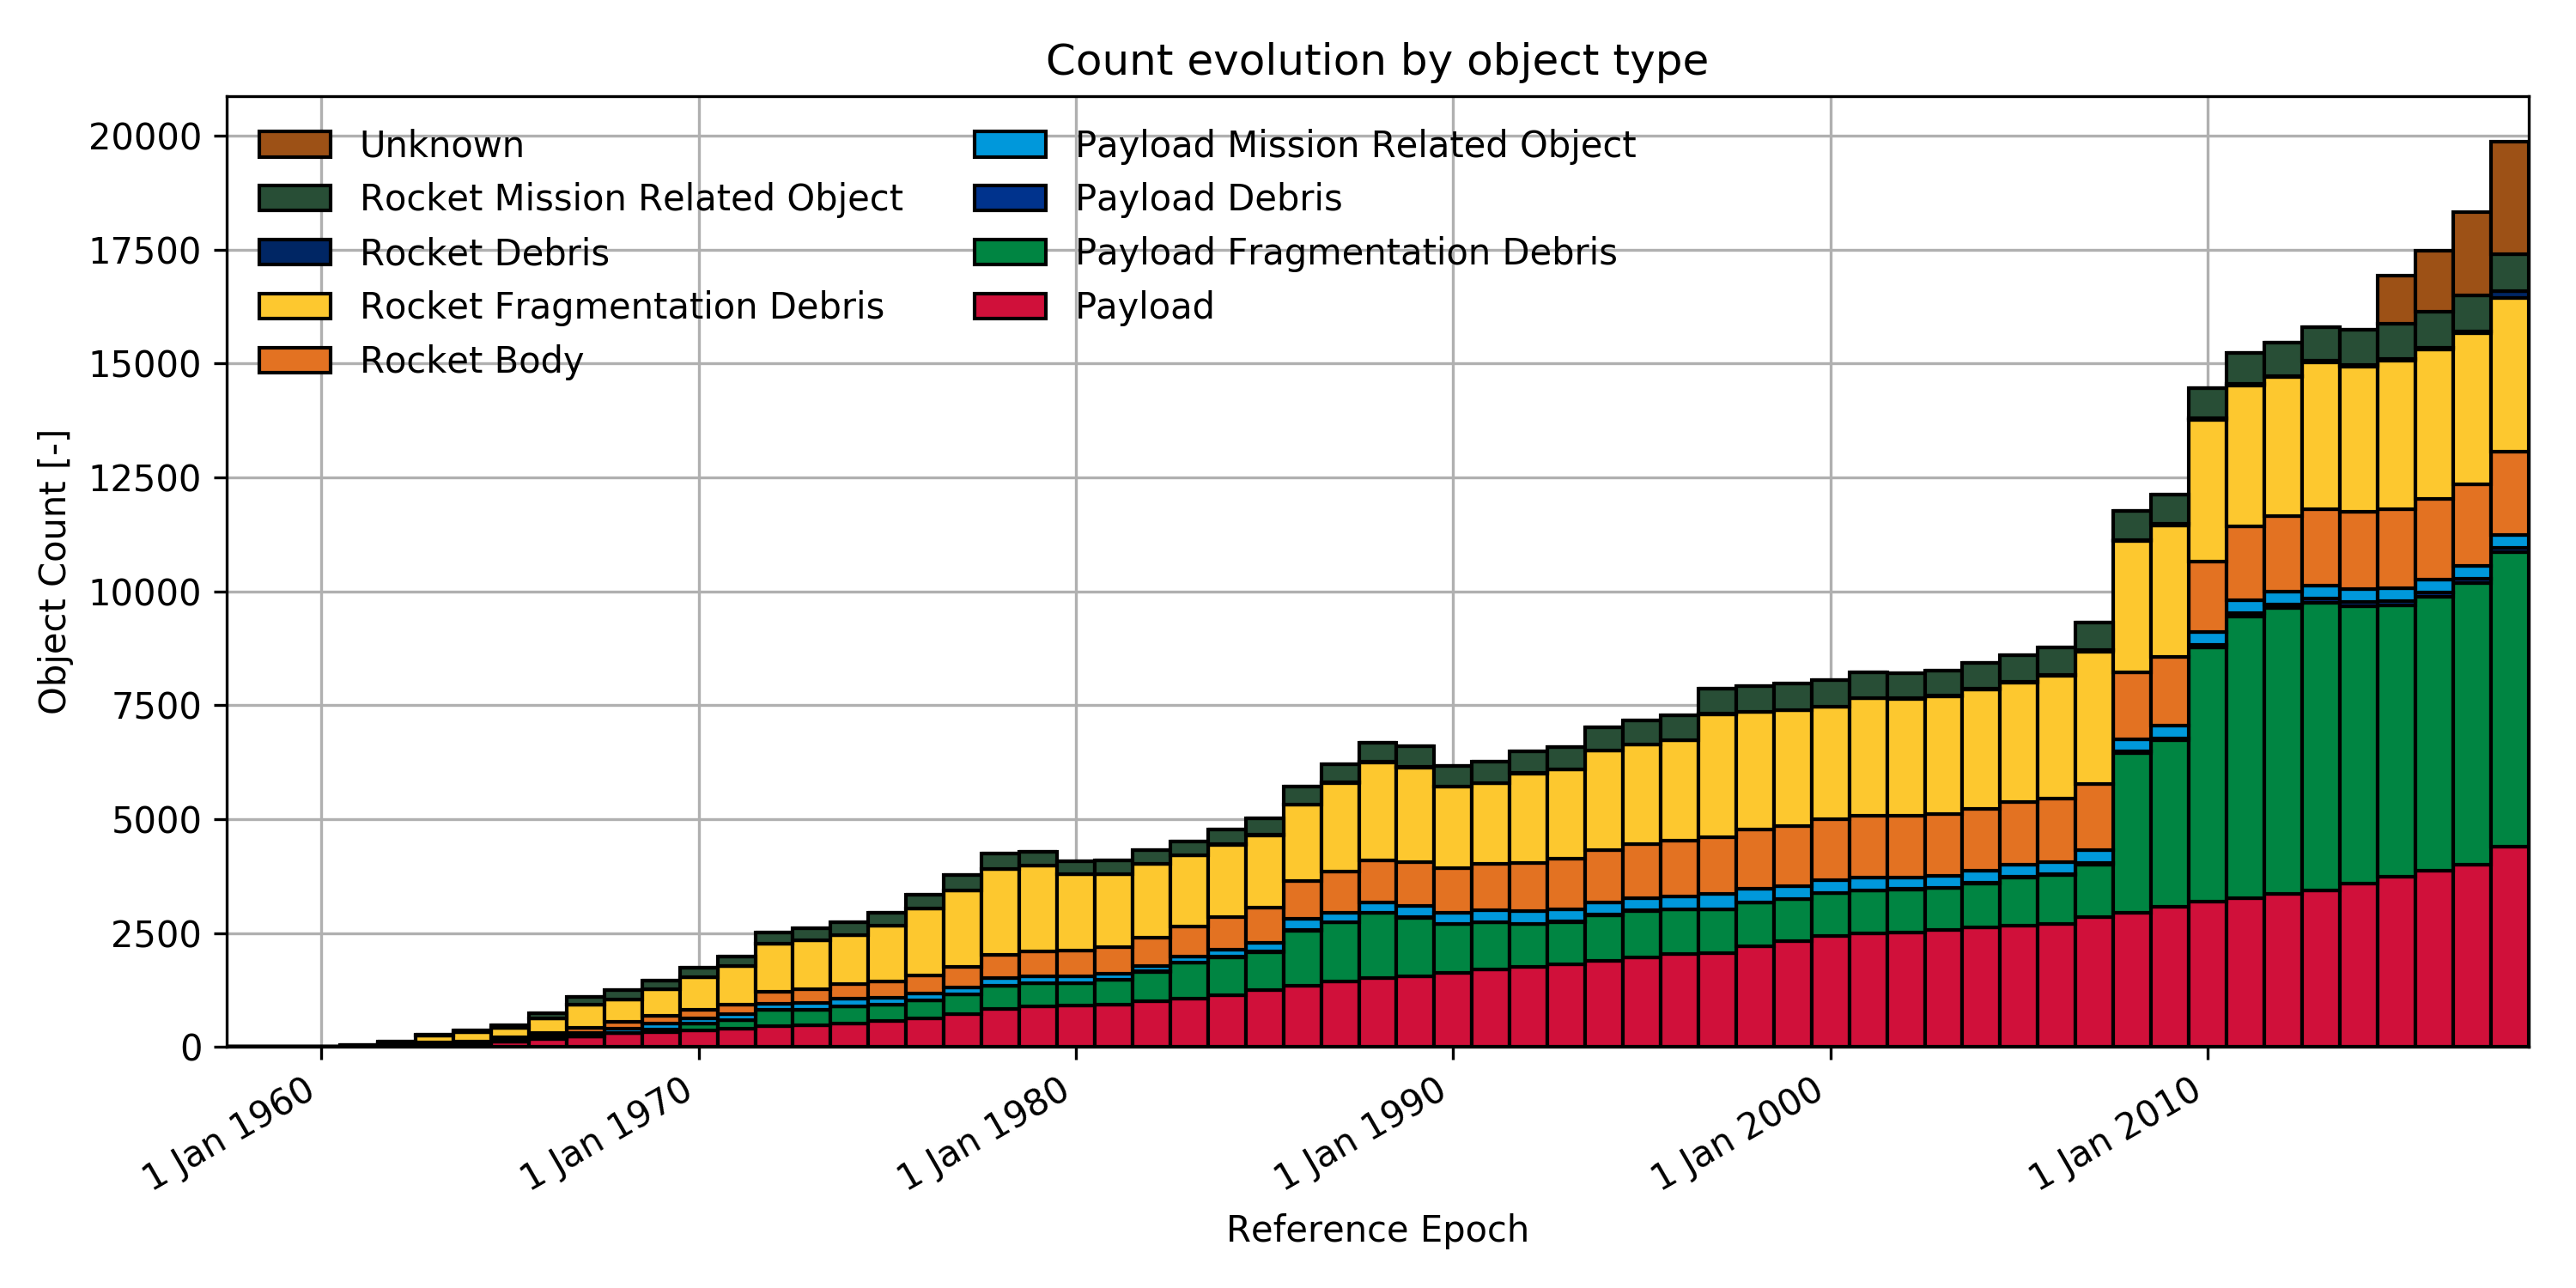
\includegraphics[scale=0.60]{images/debris_count.png}
        \label{img:debris_count}
        \caption{Evolution of debris count over time (ESA)}
    \end{center}
\end{figure}

According to the trend seen in Figure 2.1, we can clearly conclude that number of debris is rising.
Graph shows that overall count is not only rising, but it's rising trend is increasing in exponential fashion.
We can therefore conclude that while number of annual launches increases, debris count will follow the same trend.
This conclusion makes detecting of already present debris vital for slowing down the trend to avoid creating more fragmentation debris.
Our long term goal is to avoid Kessler syndrome as proposed in 1978 by NASA scientist Donald J. Kessler.
He described the consequences of a self-sustained growth of the space debris, initially triggered by collisions between intact objects and ultimately sustained by collisions between fragments.
If this scenario would become reality, it would create impenetrable barrier that would render creation of new satellites as well as exploring solar system inconceivable.

\section{Spatial distribution}

According to the first Kepler's law:

\say{Within the domain of the solar system all planets describe elliptical paths with the Sun at one focus}
\\
\\
The same law applies to geocentric motion as well meaning that any object describe elliptical path with the Earth at one focus.
\\
\\

\subsection{Types of orbits}

Objects orbiting earth can be categorized by its position as follows:
\begin{itemize}
    \item{Low earth orbit (LEO)}
    \item{Geocentric orbit (GEO)}
    \item{GNSS, GTO, Molniya}
\end{itemize}

\begin{figure}
    \centering
    \subfloat[Types of orbits]{{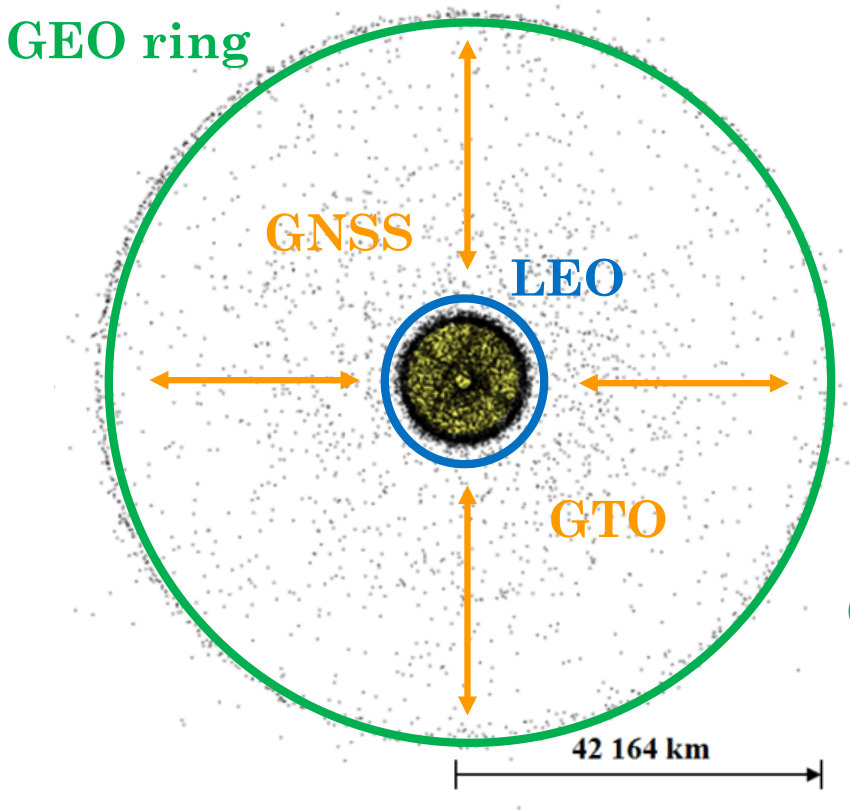
\includegraphics[width=5cm]{images/geo_leo.png} }}%
    \qquad
    \subfloat[Aproximate density]{{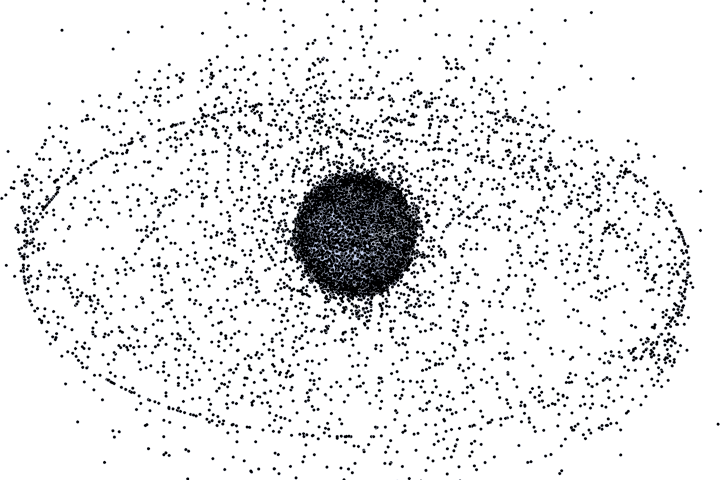
\includegraphics[width=5cm]{images/junk.png} }}%
    \caption{Space debris distribution}%
    \label{fig:example}%
\end{figure}
Low earth orbit is the most dense part of earth's orbit creating sphere-shaped layer of debris.
It consists of more than 10000 objects, mostly fragments.
\\
\\
Geocentric earth orbit, with mean altitude of 35 786km, forms ring-like shape over Earth's equator.
Cataloging objects in this orbit is more problematic and only object with size of 50cm are reflecting enough light to be detected from earth's surface.
In this thesis we will mostly focus on objects present in Low earth orbit.

\section{Data collection}

\subsection{FMPI AGO}
All the data used in this thesis is captured in Astronomical and Geophysical observatory in modra (AGO) from a main telescope with these basic features:
\begin{itemize}
    \item{Newtonian reflector with parabolic mirror}
    \item{0.7m long telescope}
    \item{2.9m focal length}
    \item{28.5x28.5 arc-min field of view}
    \item{equatorial mount}
\end{itemize}

\begin{figure}[!hbt]
    \begin{center}
        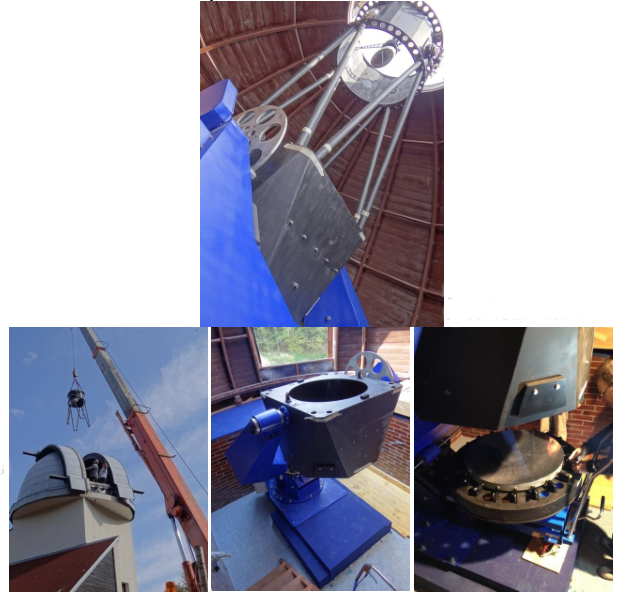
\includegraphics[scale=0.60]{images/telescope.png}
        \label{img:telescope}
        \caption{70cm telescope in AGO modra}
    \end{center}
\end{figure}

The data comes in form of 1024x1024 pixel images.

\subsection{Tracking types, fits format}
Images coming from AGO are in form of fits files (Flexible Image Transform System).
They consist of header and data.
Header contains many useful information, but for purpose of this thesis, only relevant part is type of tracking used.
We differentiate 2 types of tracking:
\begin{itemize}
    \item{Sidereal tracking}
    \item{Object tracking}
\end{itemize}

Telescope uses 5 seconds exposures and during this type it can either compensate for earths motion to remain in sync with stars in the background (sidereal) or it can move freely with earths rotation.
During sidereal tracking stars remain point-like while any object moving on earth's orbit traces streak line path.
In object tracking, polar opposite is the case.
Resulting in point in place of orbital objects, and streak lines in case of stars in the background.

\begin{figure}[!hbt]
    \begin{center}
        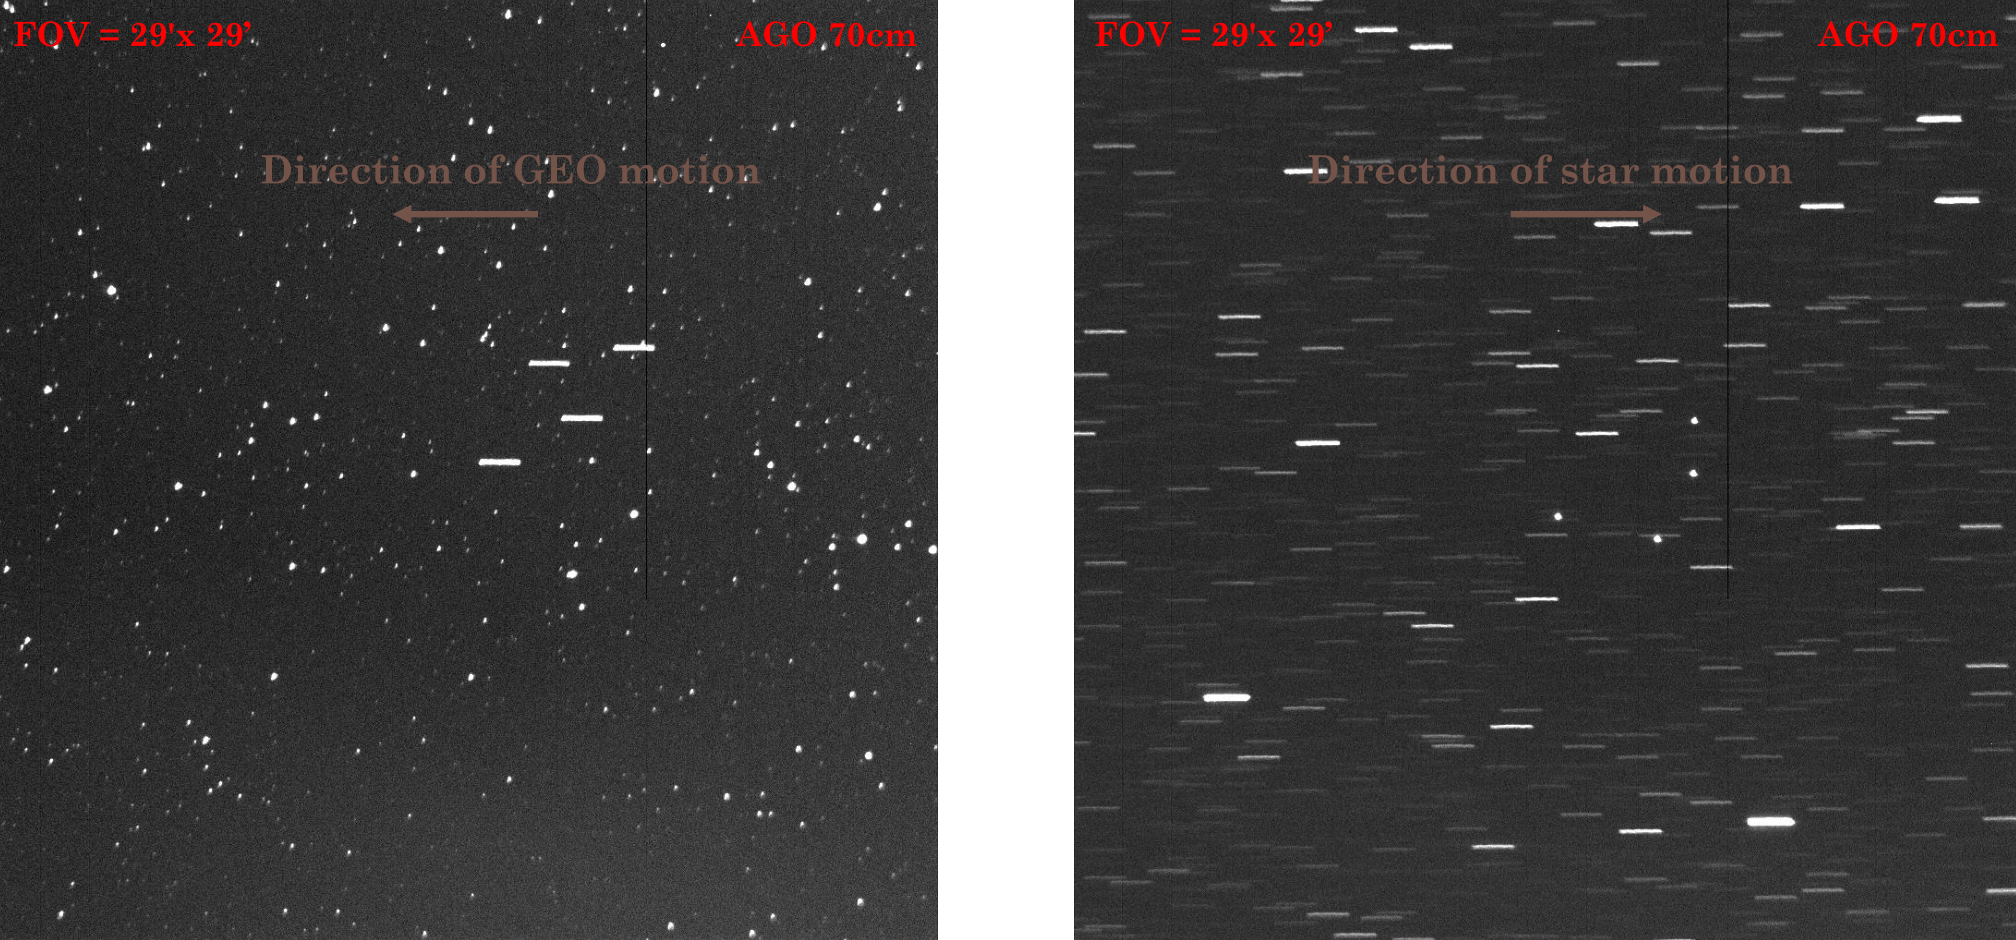
\includegraphics[scale=0.60]{images/tracking.png}
        \label{img:tracking types}
        \caption{Difference types of images with sidereal tracking (left) and object tracking (right)}
    \end{center}
\end{figure}

Data part of the fits file consists of array with size 1024x1024 containing total intensity captured during exposure.

\chapter{Processing pipeline}

\section{Pipeline definition}

The whole processing pipeline starts with capturing of image and ends with record of debris and it's RADEC coordinates.
Pipeline (as described in Slovakian Optical Sensor for HAMR Objects Cataloguing and Research) consists of following steps:
\clearpage
\begin{itemize}
    \item{Image reduction}
    \item{Sky background estimation/extraction}
    \item{Objects search and centroiding}
    \item{Star field identification}
    \item{Astrometric reduction}
    \item{Star Masking}
    \item{Tracklet building}
    \item{Object identification}
    \item{Data format transformation}
    \item{Output data redistribution}
\end{itemize}
\par
\indent
Captured image in it's raw form is not usable for later stages of pipeline, therefore it needs to be corrected first.
During image reduction, we take image with closed lid of the telescope to capture any noise created by aperture itself.
This process removes noise created by difference in sensitivity of pixels, dust present on the optical system as well as noise created by current.\\
\indent
Process of image reduction is not perfect and some noise remains, but most of the noise after this step comes from external sources.\\
\indent
Sky background estimation tries to create map of background noise.\\
After this map is created, it gets subtracted from original image, removing all global and local gradients.\\
This process can never remove all of the noise, but removing of noise gradients makes latter steps possible.\\
\indent
Star object identification takes care of locating of stars position in image coordinates(x,y).\\
These stars are then covered because their are not objects of interest.
While some stars are too weak to be labeled correctly, later processing needs to follow.\\
\indent
After stars are removed, we start segmenting objects of interest.\\
We then add another dimension to the problem, considering correlations of objects across images, across time - tracklet building.\\
\indent
The final product consists of tracklet with RADEC coordinates, therefore final conversion from image coordinates(x,y) is needed.\\

\section{Sky background estimation and extraction}
While a lot of a noise present in captured images is coming from aperture itself and is removed in early stages of processing, external sources cannot be removed in the same way.
There are several sources of external noise:
\begin{itemize}
    \item{Moon light (global linear gradient)}
    \item{Stars, Nebulas, Galaxies (local nonlinear gradients)}
    \item{Remnants of hardware related reflections}
\end{itemize}
Two basic algorithms are used to extract background from image.

\subsection{Median filtering}

This method is very simplistic, but suffers few disadvantages.
Idea behind this method is to use 2-d convolution with median kernel of size at least 0.2 times original image.
As a result of this convolution process, blurred version of original image is being created.
Main advantage of this method is that it preserves faint objects and original noise and this effect increases with use of larger kernel sizes.
Obvious disadvantage of this method is that if we want to achieve usable results, large kernel needs to be used and this increases computation time exponentially.Version of this algorithm was implemented during this thesis but to archive any usable results, 20 to 30 seconds were spent in convolution computation.
This timespan is unacceptable when considering whole pipeline length.
Another disadvantage of this method is that it doesn't detect small local gradients and this effect only increases with kernel size.
The last but not least problem with this approach comes from very nature of convolution and with it's behavior near edges of image.
Image after this process loses data on border of image with width of half of kernel size.

\subsection{Sigma clipping}

Sigma clipping takes different approach.
It consists of preprocessing and iterative clipping process (As described in Distinguishing features of CCD astrometry of faint GEO objects, Vladimir Kouprianov 2007).
We first need to define some parameters and other values used in this method.
\begin{itemize}
    \item{$\sigma$ - standard deviation}
    \item{$\overline{\Delta B_i}$ - mean deviation}
    \item{I(x,y) - intensity of pixel x,y of original image}
    \item{$B_0$(x,y) - intensity of pixel x,y of initial background estimate}
    \item{$B_i$(x,y) - intensity of pixel x,y of i-th iteration of background map}
    \item{B(x,y) - intensity of pixel x,y of resulting background map}
\end{itemize}

\subsubsection{Image preprocessing}
Sigma clipping method iteratively converges to background map, but firstly it needs initial estimation to iterate over.\\
The initial estimation is created by downsizing of the image to 10\% of the original size using bicubic interpolation.\\
This helps with minimizing of aliasing artifacts.
After that we blur the downsized image with median filter, but in contrast to median filtering method, we use much smaller kernel size.
Next we upsize the image and smooth it out with gaussian filter convolution.\\
The resulting image is then used in next step of the algorithm.

\begin{figure}[!hbt]
    \begin{center}
        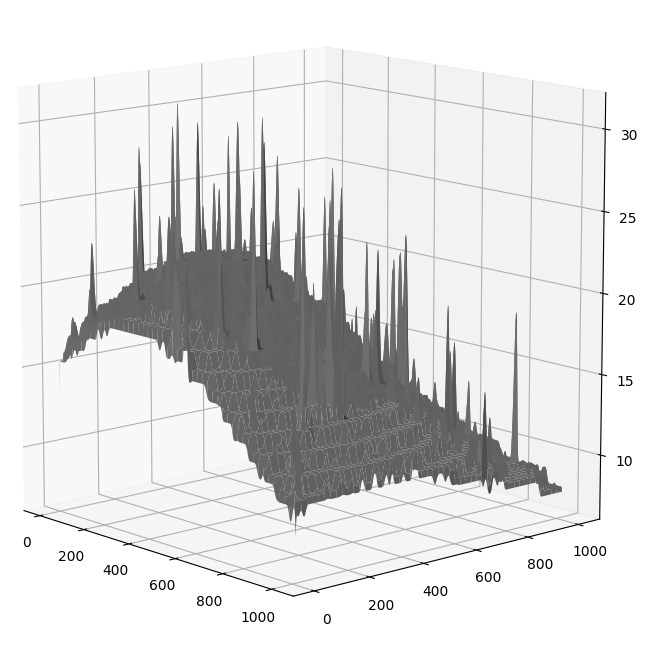
\includegraphics[scale=1.30]{images/background_initial_guess.png}
        \label{img:background_initial_guess}
        \caption{Map produced by initial estimation}
    \end{center}
\end{figure}

\subsubsection{Iterative process}
Preprocessed image already shows the global background trend, but it is far from being usable in this form.\\
We iterate the image with following equation: \\
\begin{gather}
    \Delta B_{i+1} =
    \begin{cases}
        \Delta B_i(x,y) & |\Delta B_i(x,y)-\overline{\Delta B_i}| < 3\sigma_i\\
        \overline{\Delta B_i}& |\Delta B_i(x,y)-\overline{\Delta B_i}| >= 3\sigma_i\\
    \end{cases}
\end{gather}

The equation has 2 cases to consider depending on the difference between value of previous iteration (or estimated value in first iteration) and mean deviation compared with standard deviation.\\
The final product of background map is then computed with $n$ iteration as
\begin{equation}
    B(x,y) = B_0(x,y) + \Delta B_n(x,y)
\end{equation}

\begin{figure}[!hbt]
    \begin{center}
        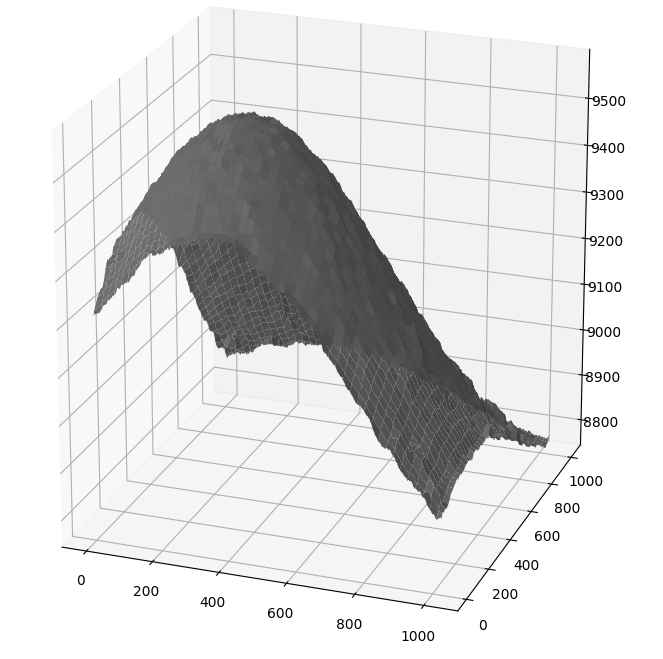
\includegraphics[scale=1.50]{images/3_iter_sigma.png}
        \label{img:background_initial_guess}
        \caption{Final result with 3 iterations}
    \end{center}
\end{figure}

Compared to median filtering this algorithm produces background image faster and it's speed can be modified with proper choice of number of iterations.

\subsubsection{Parameter choice}
During implementation we experimented with all the parameters of the algorithm to obtain the best results possible.
We experimented with different sigma values used in case equation(3.1) as well as changing of mean derivation to median derivation.\\
Changes showed some promising results on test cases, but parameters being described above showed to be the most robust.\\
We also experimented with choice of preprocessing steps.
Best results were obtained with choice of kernel with size of 15x15.
This parameter choice showed best trade-off between speed of computation and minimizing artifacts on the resulting map.\\
Lastly we considered blurring the resulting image with gaussian blur to completely remove any artifacts that could be produced during iteration.
This showed to be quite difficult choice to make since it increases smoothness of the result but the choice of kernel distorts result smoothing out small gradients.
Therefore this idea was implemented as an optional choice in the final implementation.\\

\clearpage
\begin{figure}
    \centering
    \subfloat[3 iterations]{{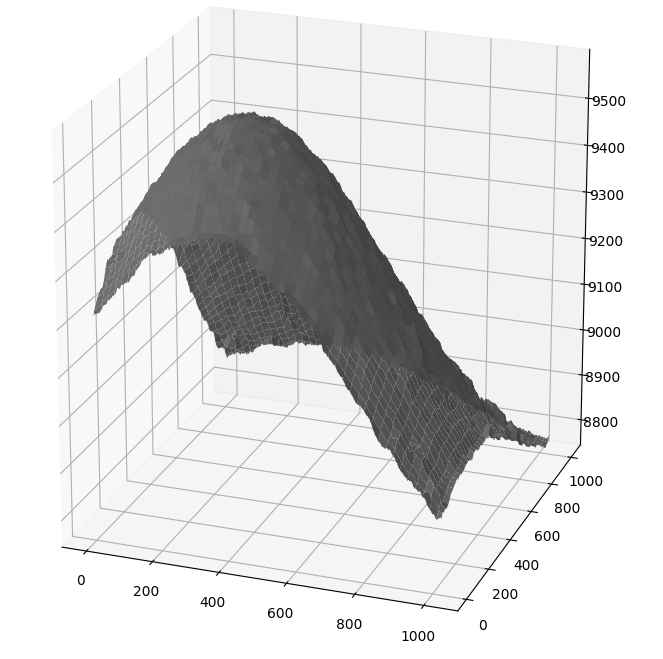
\includegraphics[width=5cm]{images/3_iter_sigma.png} }}%
    \qquad
    \subfloat[5 iterations]{{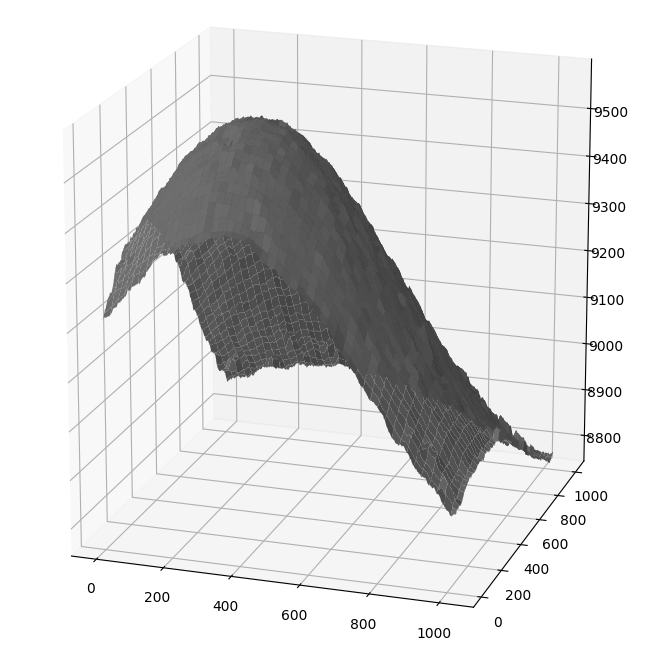
\includegraphics[width=5cm]{images/5_iter_sigma.png} }}%
    \qquad
    \subfloat[7 iterations]{{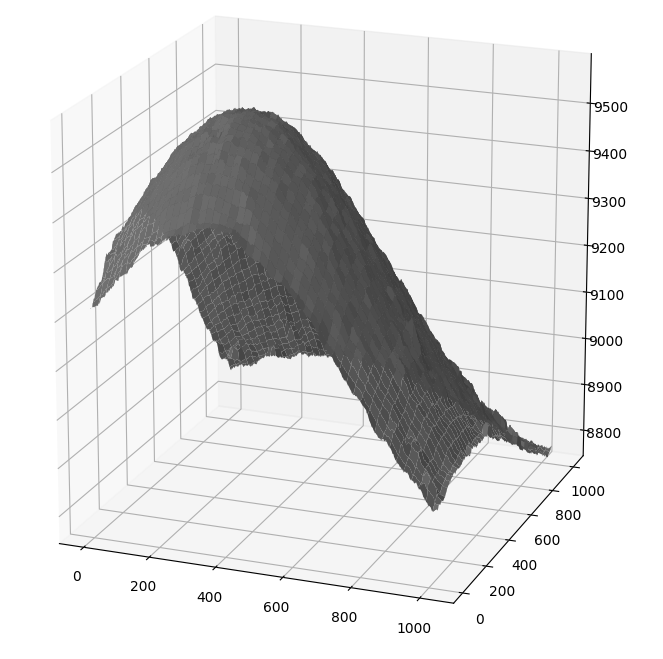
\includegraphics[width=5cm]{images/7_iter_sigma.png} }}%
    \qquad
    \subfloat[13 iterations]{{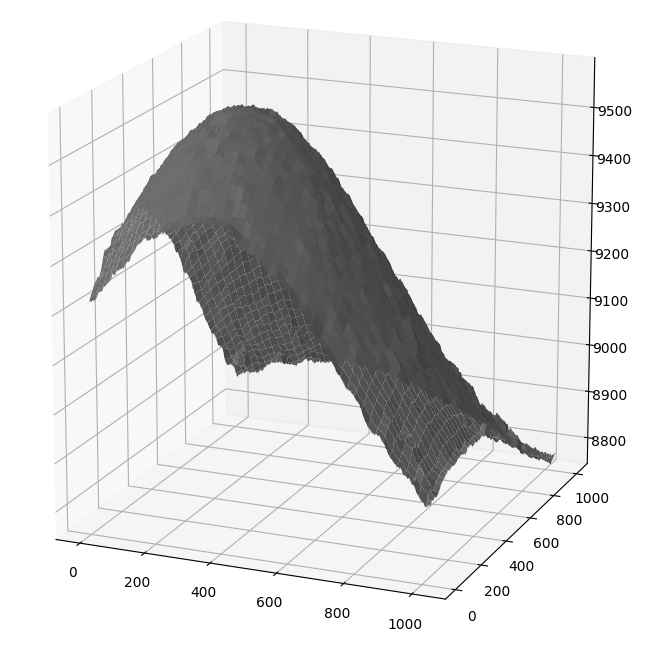
\includegraphics[width=5cm]{images/13_iter_sigma.png} }}%
    \caption{Comparison of different choice of number of iterations}%
    \label{fig:iterations}%
\end{figure}

We can observe (from Figure 3.3 and Table 3.1) that increasing number of iterations after some threshold doesn't affect results.\\
The biggest changes occur in first iterations and every iteration after third changes sigma negligibly.\\
Every image is unique, therefore in the final implementation, number of iterations is parameter to choose, but 3 iterations seem to be reasonable default value.

\begin{table}[]
    \centering
\begin{tabular}{|l|l|}
\hline
                  & sigma               \\ \hline
after iteration 1 & 327.22663761177654 \\ \hline
after iteration 2 & 248.90467048529462 \\ \hline
after iteration 3 & 248.2559262263531  \\ \hline
after iteration 4 & 248.2559262263531 \\ \hline
\end{tabular}
    \caption{Change of sigma after iterations}
    \label{tab:sigma}
\end{table}

\subsection{Grid sigma clipping}
During implementation we considered use of sigma clipping in different manner.
The core idea was splitting the image into sections generating $n$ columns and $m$ rows.
This approach creates $n \times m$ sub-images each with size
\begin{equation}
    (width_{original}/n) \times (height_{original}/m)
\end{equation}
with and possible extra pixel in last row (or column depending on considered dimension) if size of the image is not even.
The main hope behind this approach was to make sigma clipping algorithm more robust to small background gradients with added option to choose these parameters.
This would give us option to detect even the smallest of background phenomena.
Version of this algorithm was implemented during the implementation part of the this thesis.


\clearpage
\begin{table}[]
    \centering
\begin{tabular}{|l|l|l|}
\hline
                  & absolute difference & mean difference\\ \hline
    no grid & 97969264.02840663 & 93.47484103256222 \\ \hline
    10x10 & 98015474.91055997 & 93.43077090111412 \\ \hline
    30x30 & 97968103.14388879 & 93.42966379536513  \\ \hline
    50x50 & 97976495.76744124 & 93.43766762489437 \\ \hline
\end{tabular}
    \caption{Absolute and mean difference between background generated by algorithm (with multiple grid variations) and original synthetic background}
    \label{tab:grid_results}
\end{table}


As observed by absolute difference metric in Table 3.2, this approach shows bigger absolute difference then original non-grid version, but only at small grid numbers. Nevertheless grid version outperformed non-grid version on $30 \times 30$ run.
We can see some improvement but it comes with a cost.
Separation of the image into smaller segments takes extra time although performance hit is minimal.
Real negative side of this approach lays in the last part of the process, joining all the pieces of background back together.
This creates step-like relics on lines where image was cut.
These relics demand another smoothing at the end to fix this irregularity, distorting data.
Clearly, some improvement can be achieved but improvement is minimal.

\begin{figure}[!hbt]
    \begin{center}
        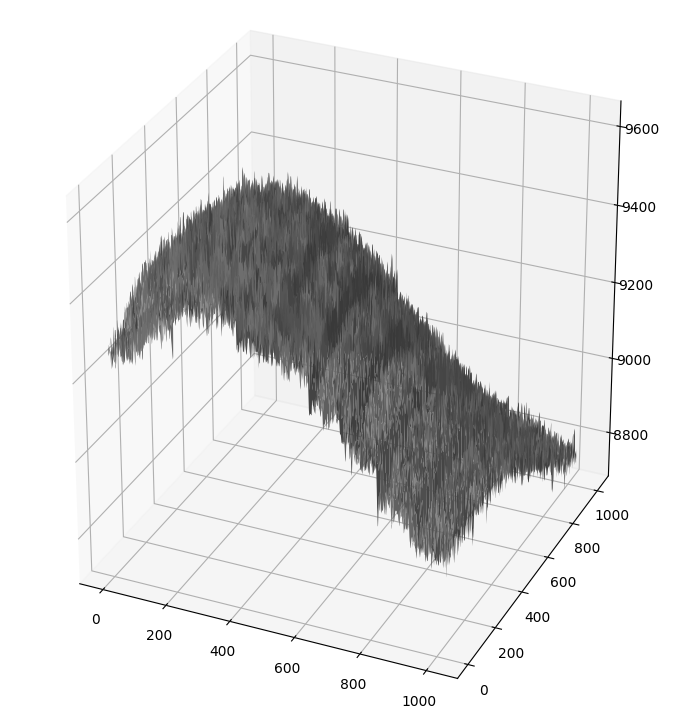
\includegraphics[scale=0.50]{images/grid_steps.png}
        \label{img:grid_steps}
        \caption{Grid steps, joining artefacts ($10 \times 1$ grid)}
    \end{center}
\end{figure}

In Figure 3.4 we can observe steps before smoothing, clearly showing additional data distortion.
Example used $10 \times 1$ to make steps more visible.


\backmatter

\bibliographystyle{alpha}
\bibliography{references}

\listoffigures

\end{document}
